\documentclass{article}
\usepackage{graphicx}
\usepackage{float}
\usepackage[spanish]{babel}
\usepackage{hyperref}
\usepackage{csquotes}
\graphicspath{ {img/} }
\setlength{\parskip}{\baselineskip}

\title{Areas Recreativas - Final \\[3ex] \small PAMN - Programación de Aplicaciónes Moviles Nativas}

\author{Chamil José Cruz Razeq}

\begin{document}
    \maketitle
    \thispagestyle{empty}
    \newpage

    \section{Introducción}

    Todos los informes sobre las tareas propuestas se encuentran disponibles en el
     siguiente repositorio de \href{https://github.com/chamilstudy/ulpgc_pamn_labs}{GitHub}
     y la aplicación se encuentra en \href{https://github.com/chamilstudy/pamn_proyecto_final}{GitHub}.

    Este documento recoge la información referente al final del desarrollo de la
     aplicación de Areas Recreativas.

    \section{Cambios Realizados}

    Se ha debugueado la aplicación implementando circulos de carga y pantallas de transición.
    
    Además se ha implementado en el fichero "strings.xml" todas las ristras utilizadas en
     la aplicación, para facilitar una posible localización de la aplicación en otro idioma.

    \section{Reparto de tareas}

    Todas las tareas serán desarrolladas por el autor de este documento.

    \section{Muestra de desarrollo}

    \begin{figure}[H]
        \centerline{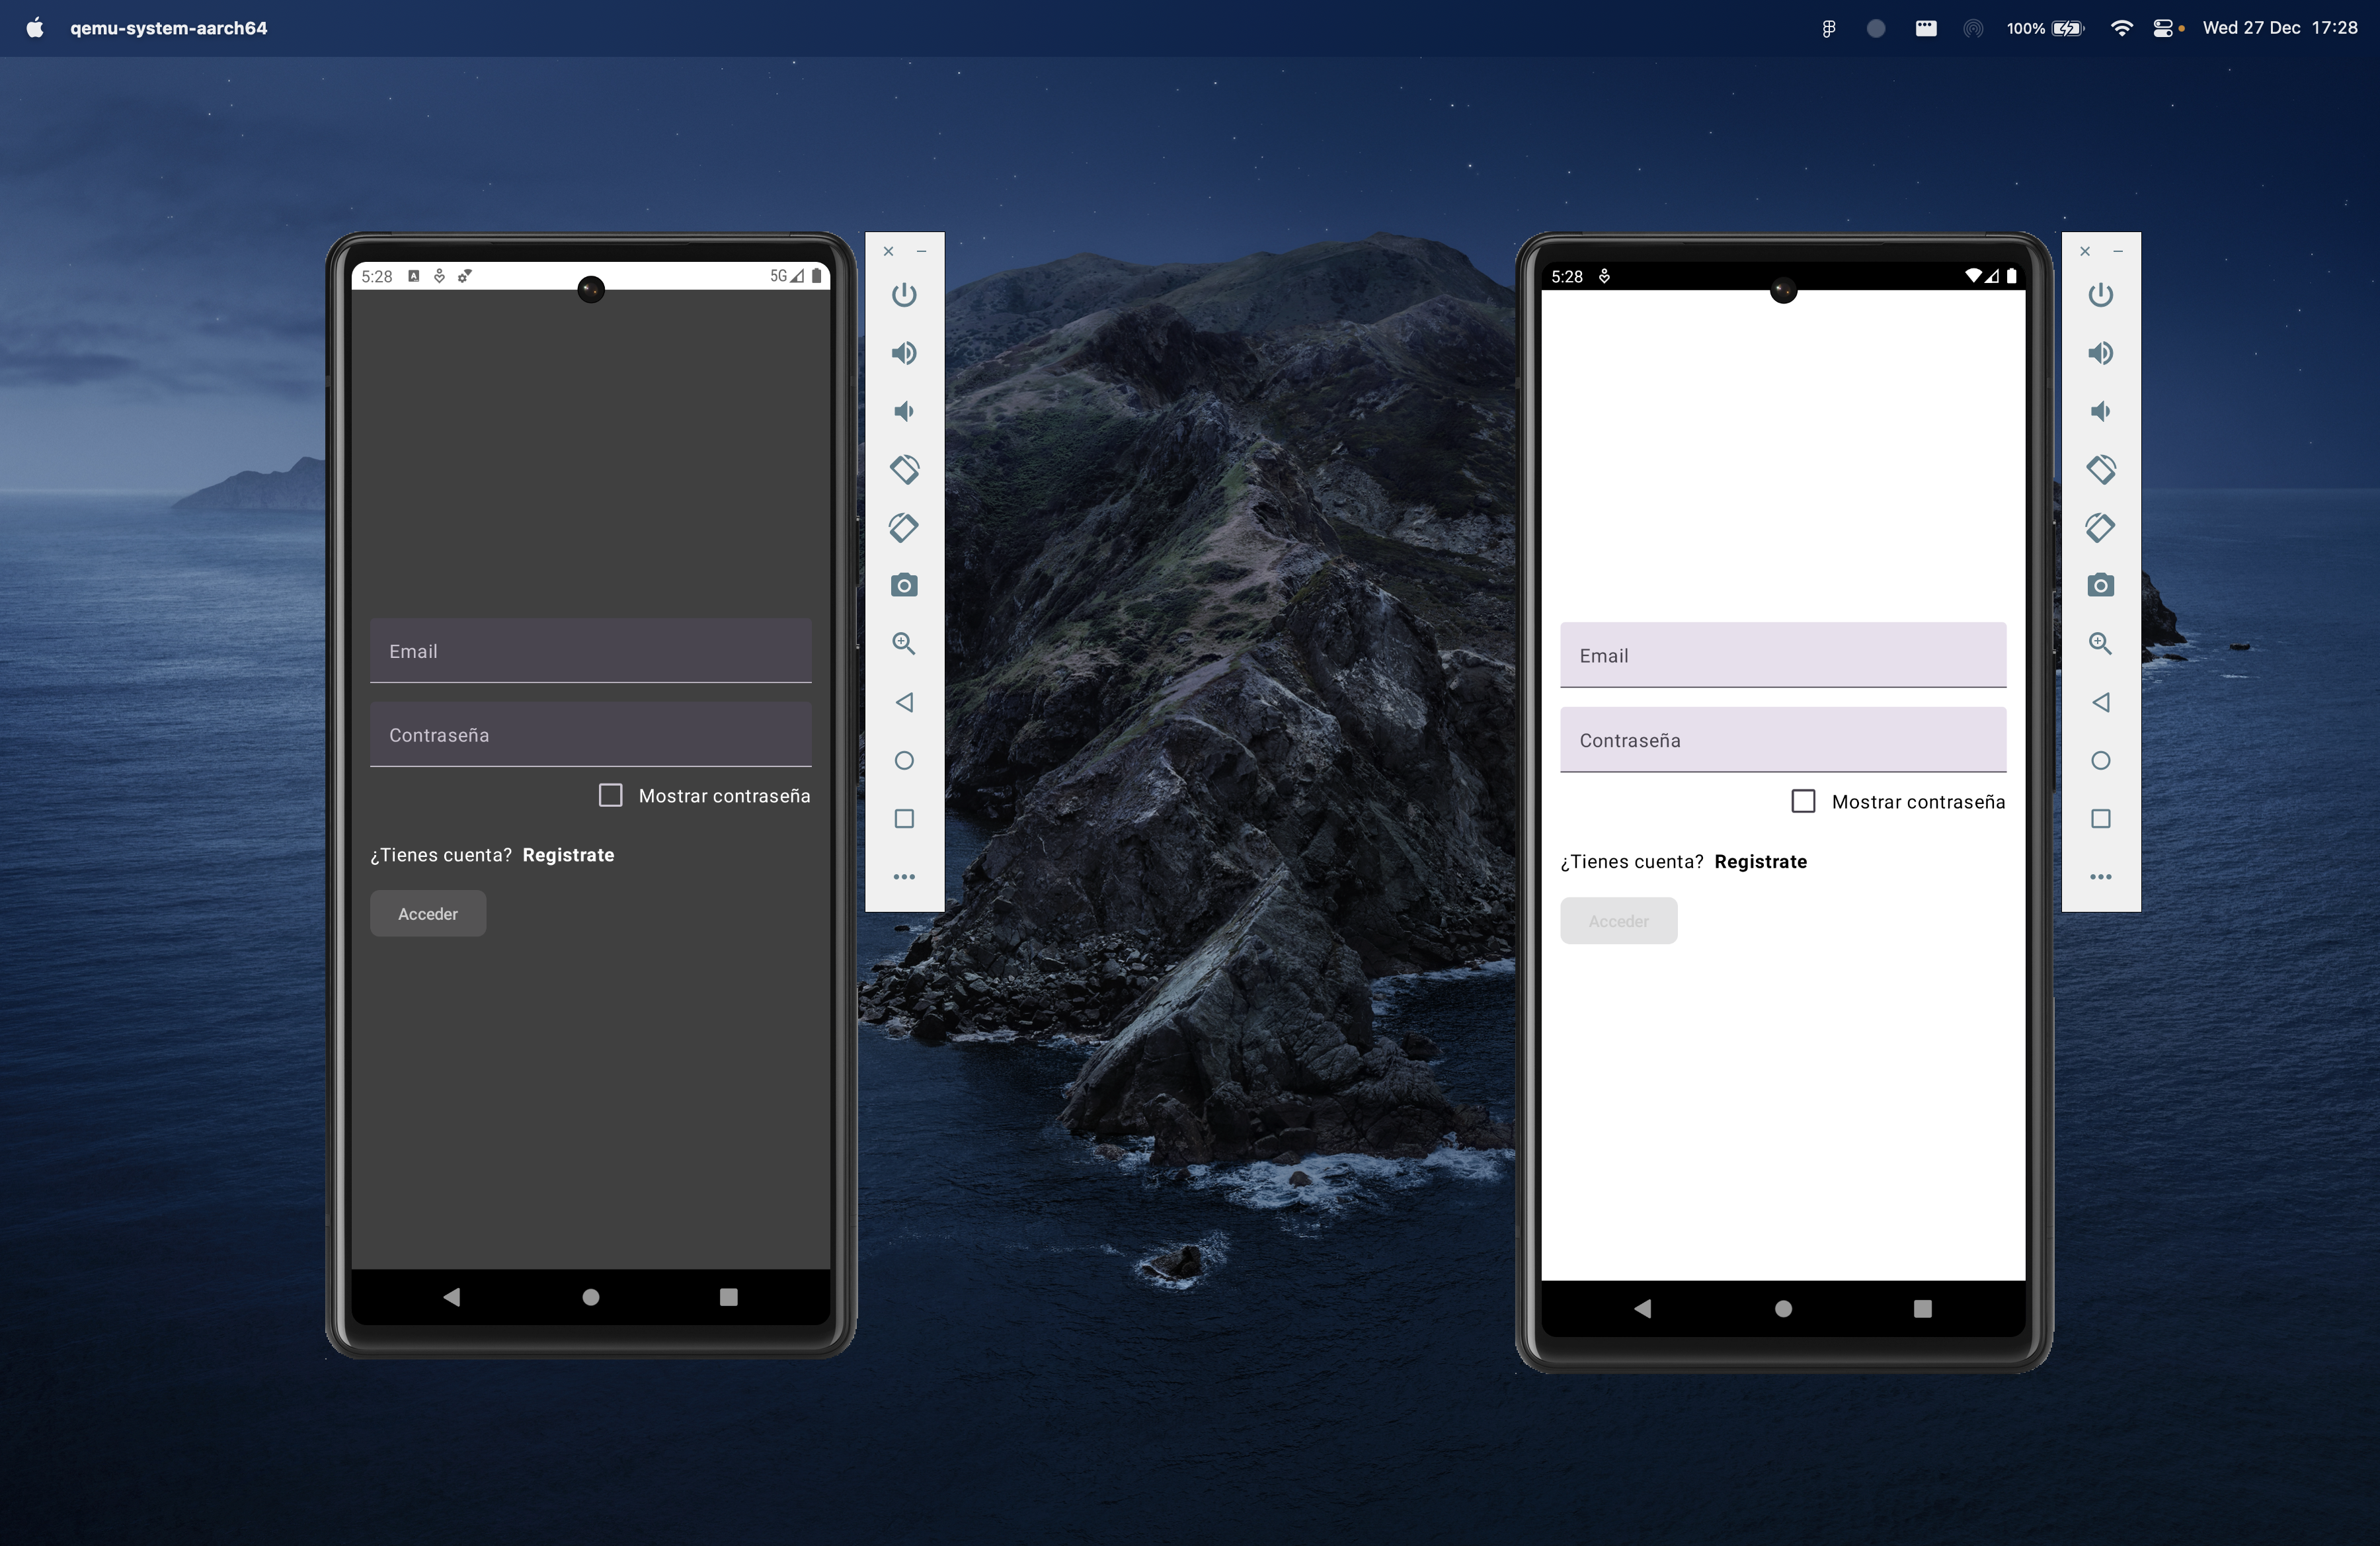
\includegraphics[scale=0.2]{login.png}}
        \caption{Login principal}
        \label{fig:login}
    \end{figure}

    \begin{figure}[H]
        \centerline{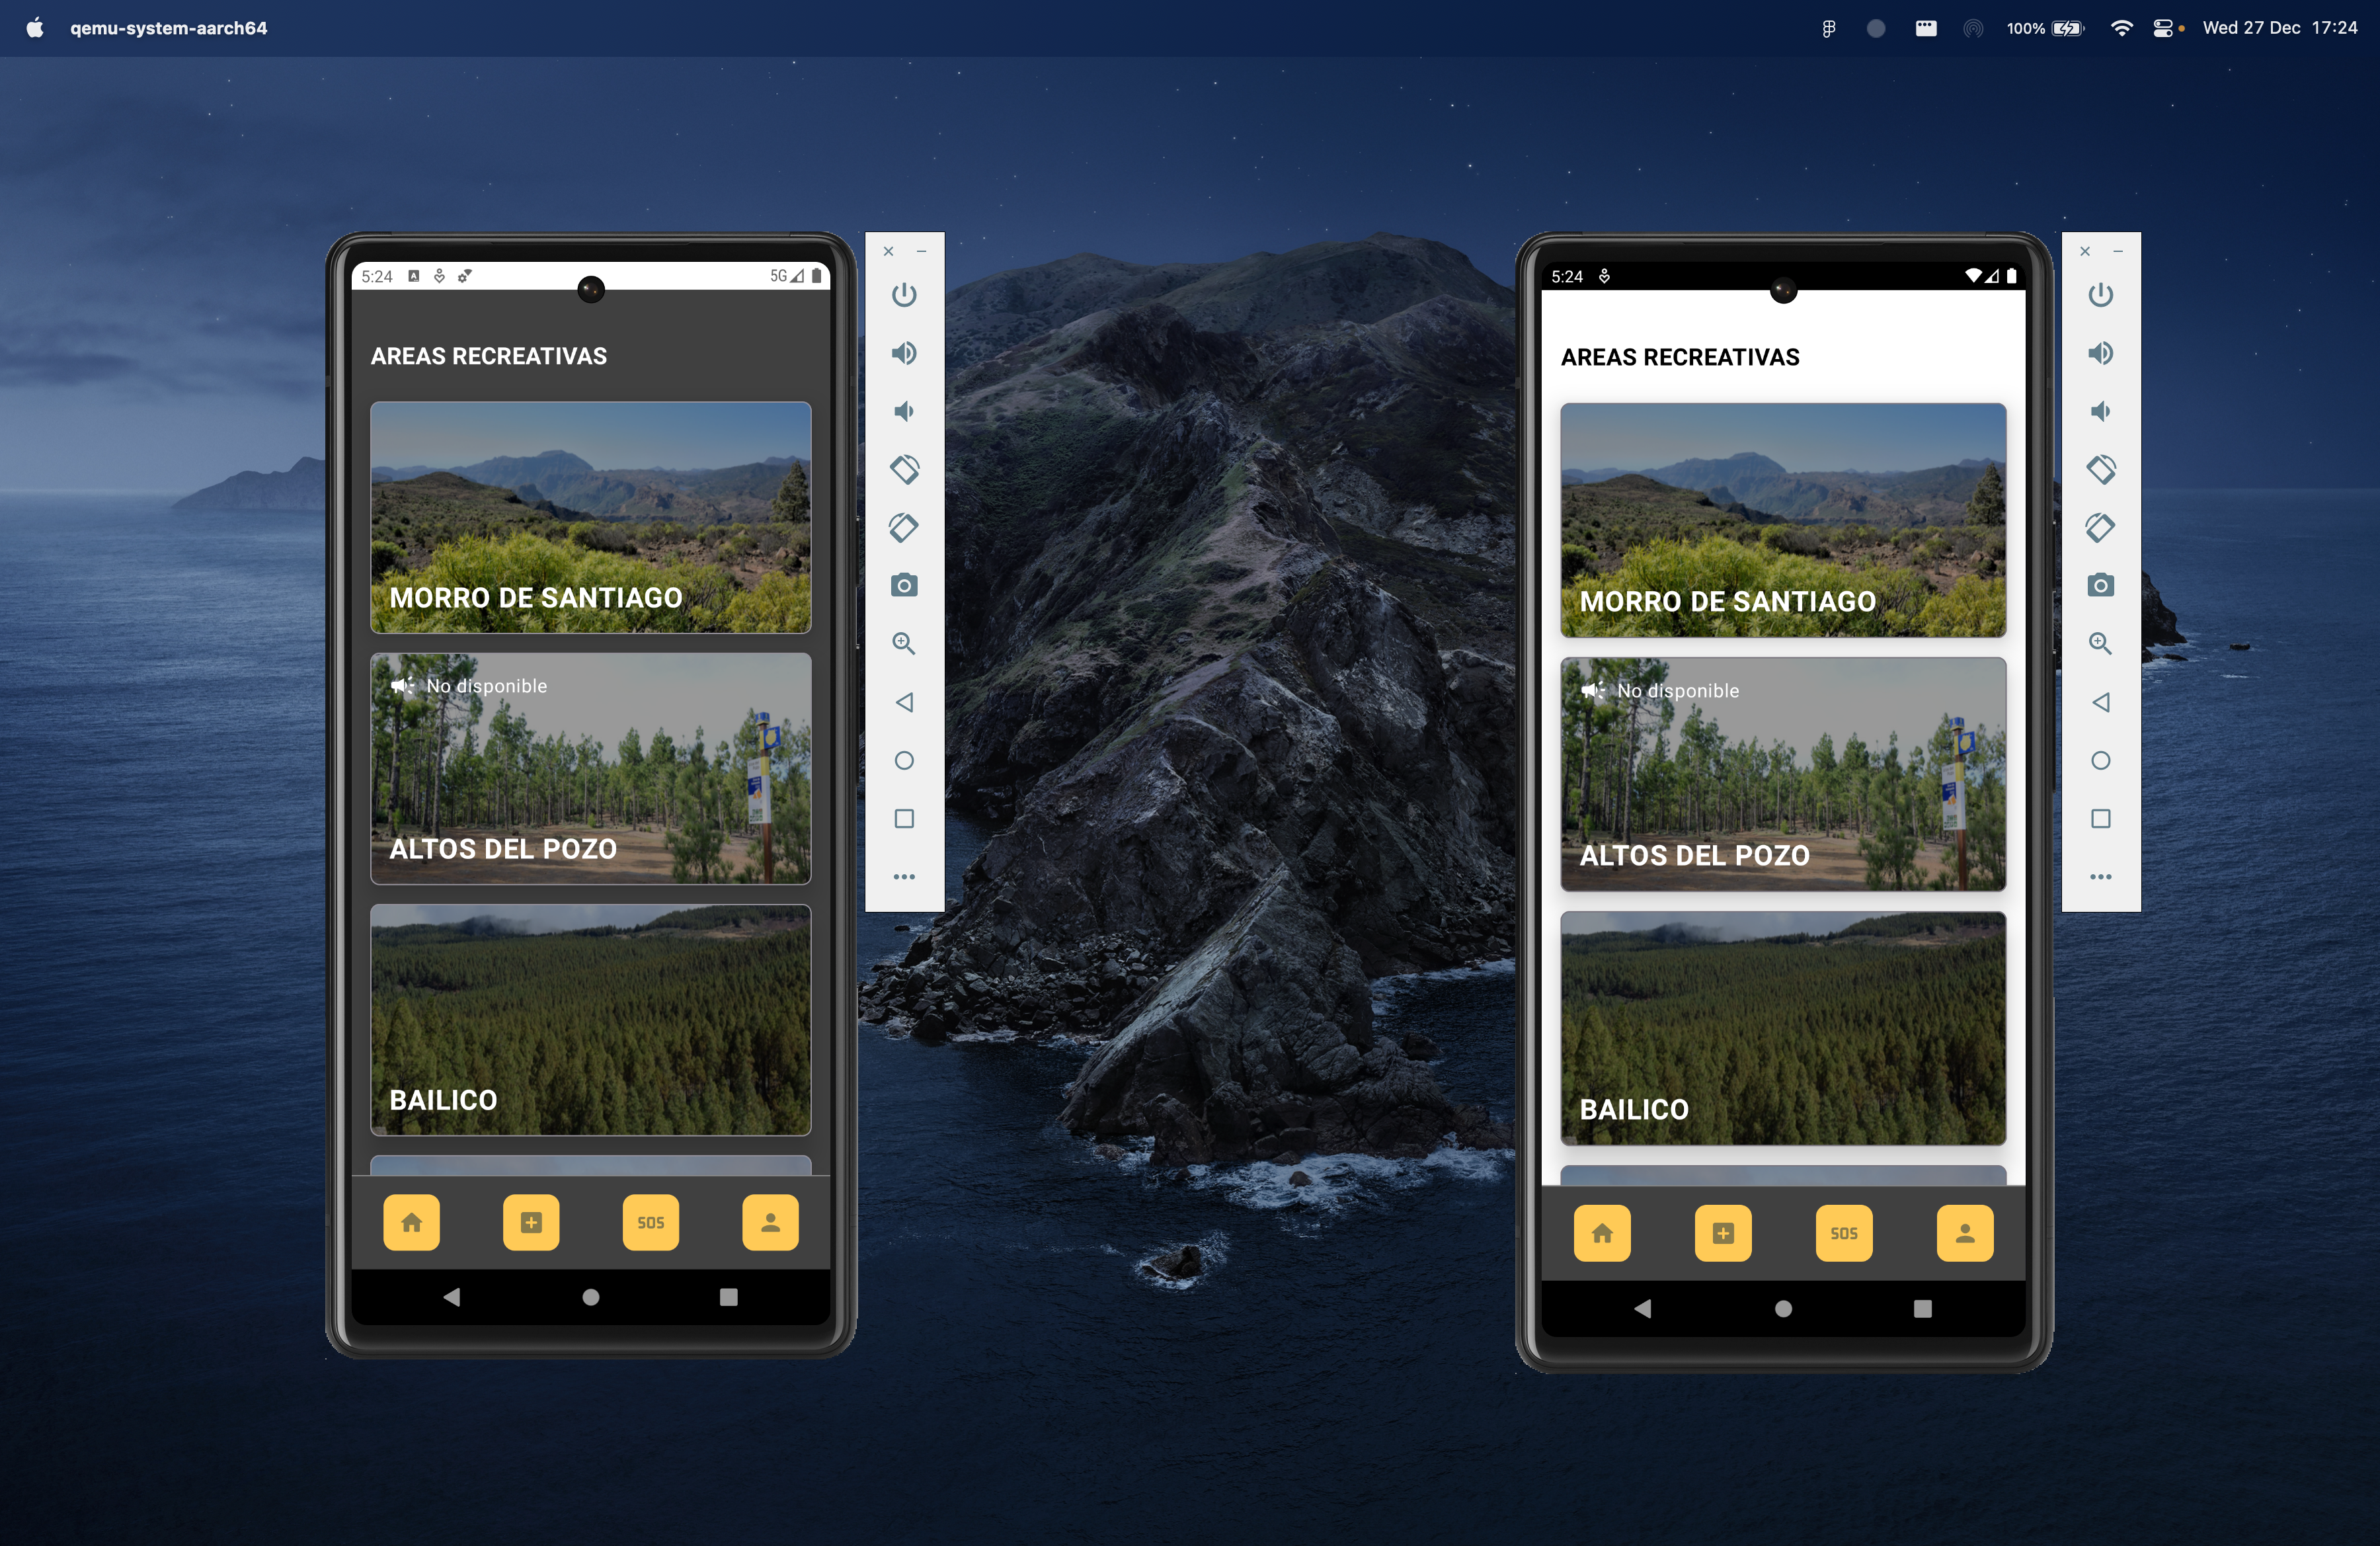
\includegraphics[scale=0.2]{home.png}}
        \caption{Pantalla principal}
        \label{fig:home}
    \end{figure}

    \begin{figure}[H]
        \centerline{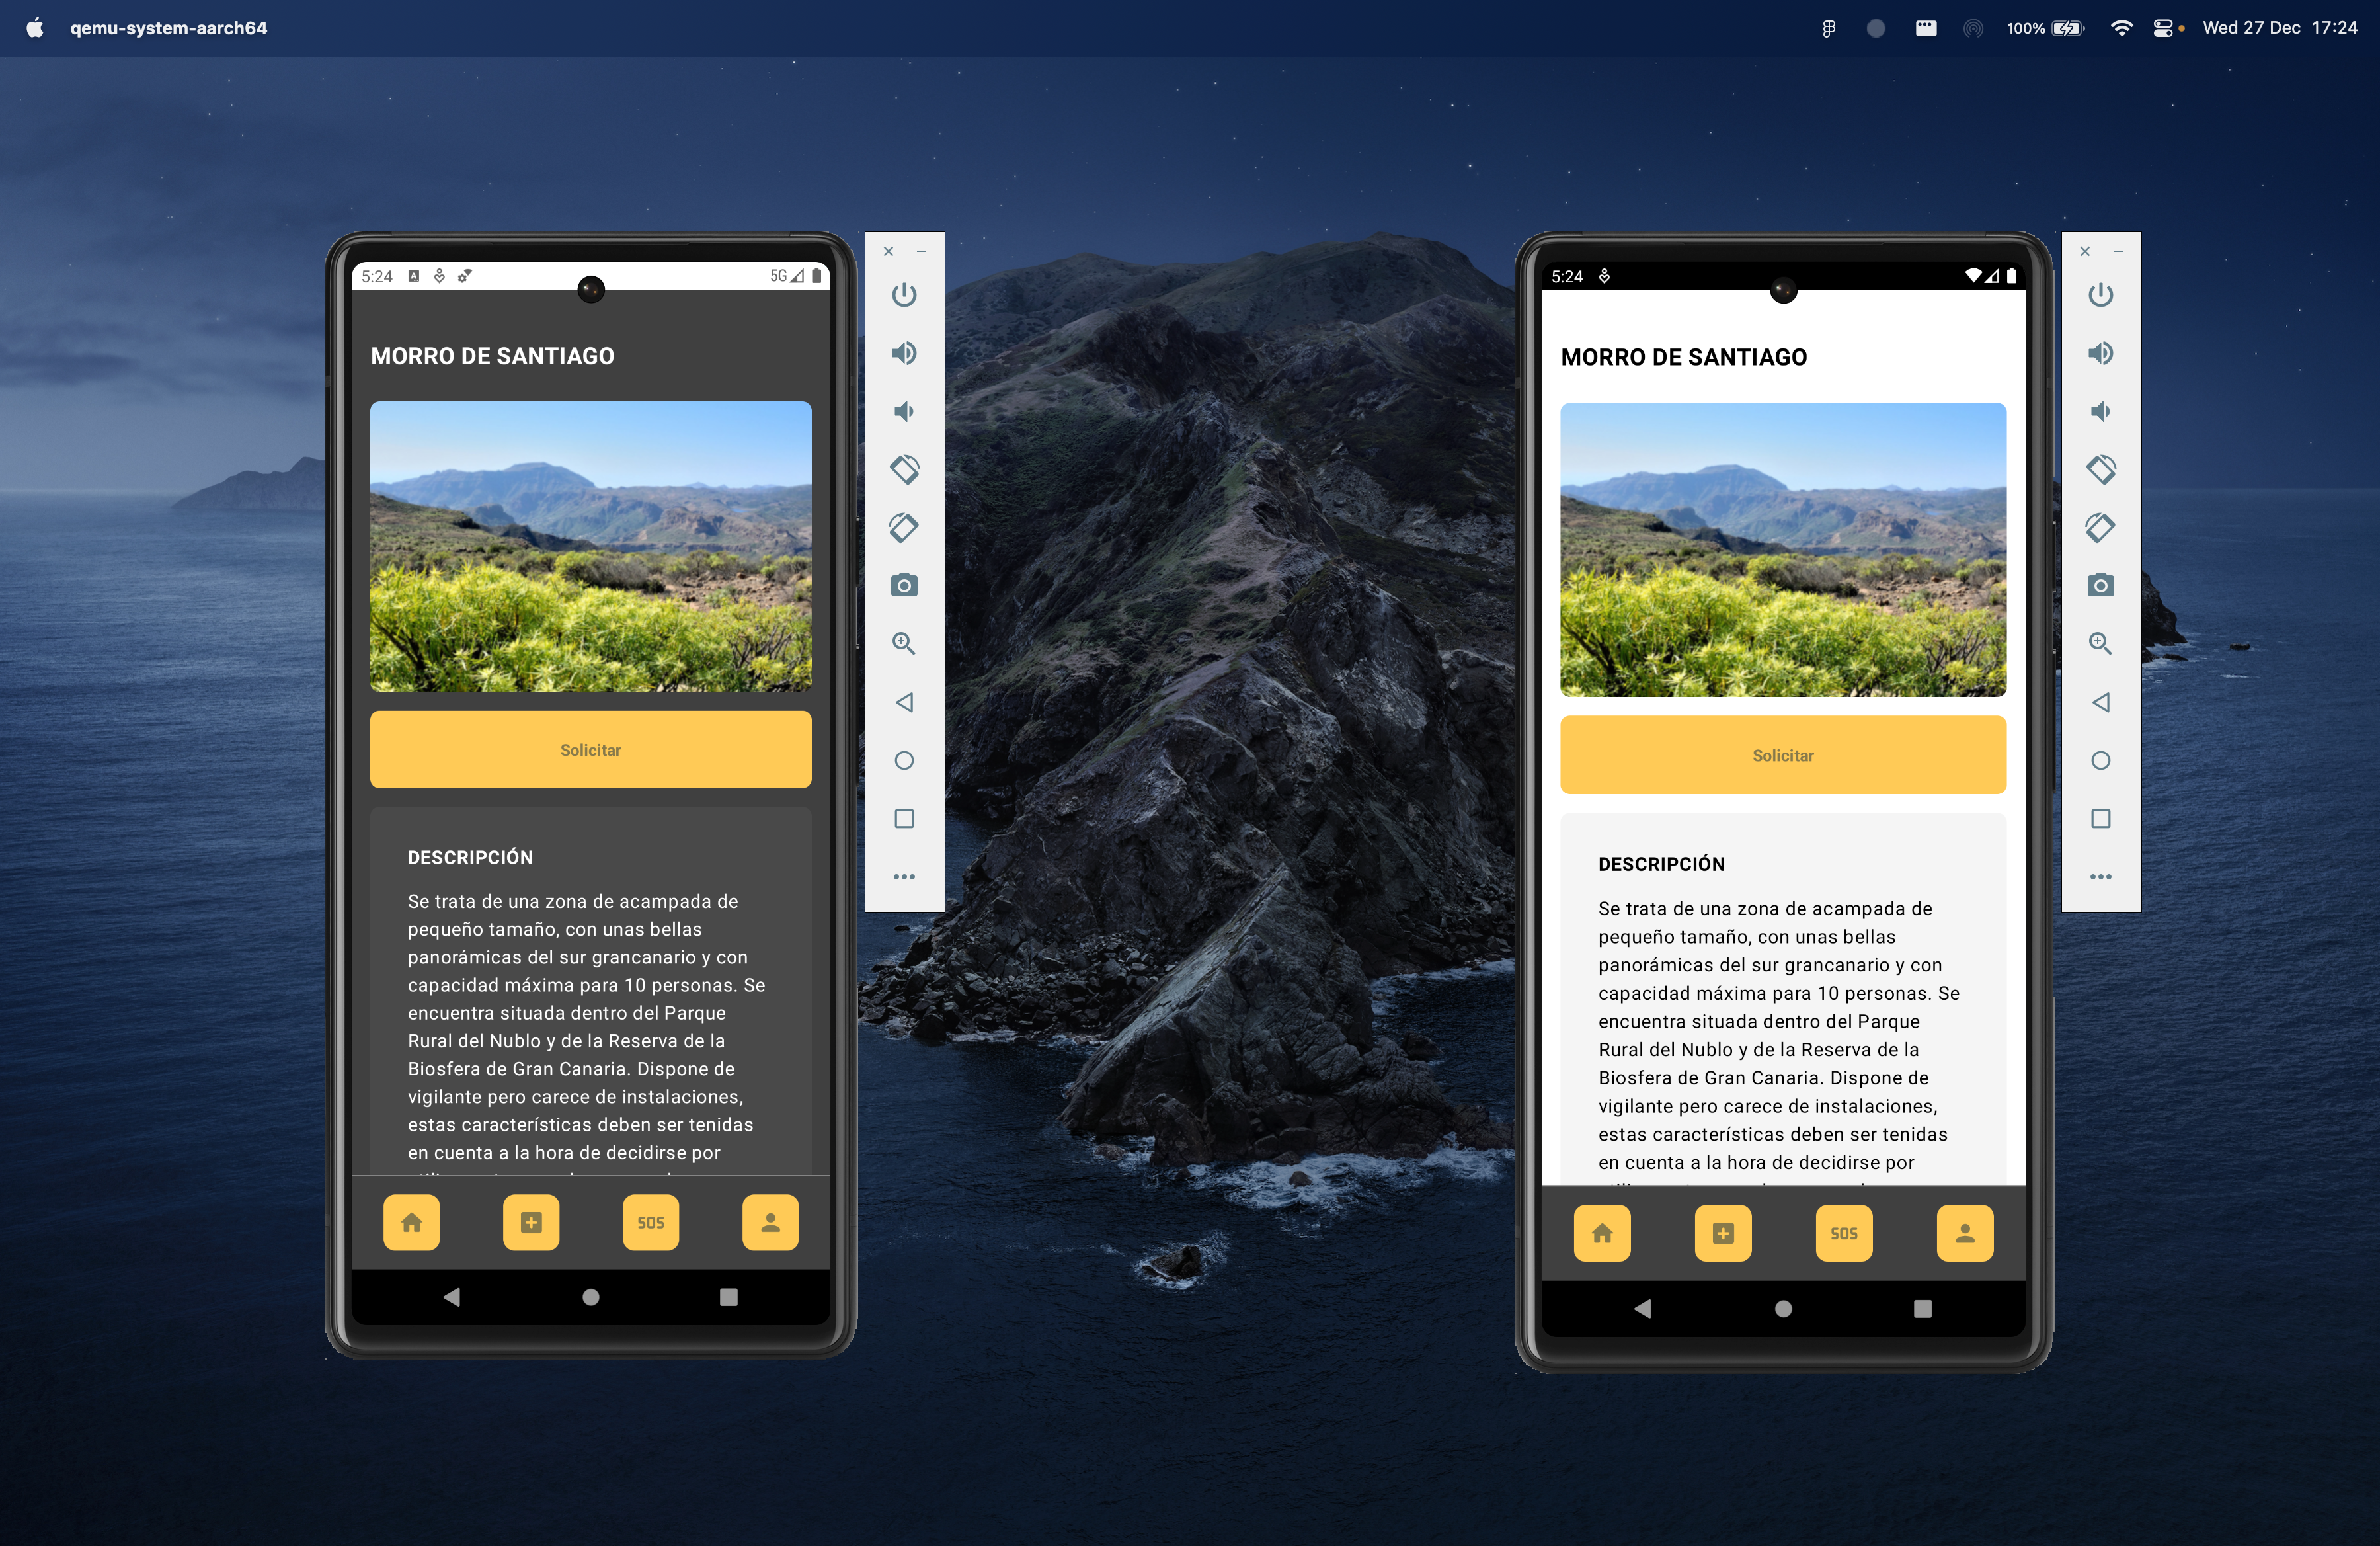
\includegraphics[scale=0.2]{area1.png}}
        \caption{Pantalla de area seleccionada}
        \label{fig:area1}
    \end{figure}

    \begin{figure}[H]
        \centerline{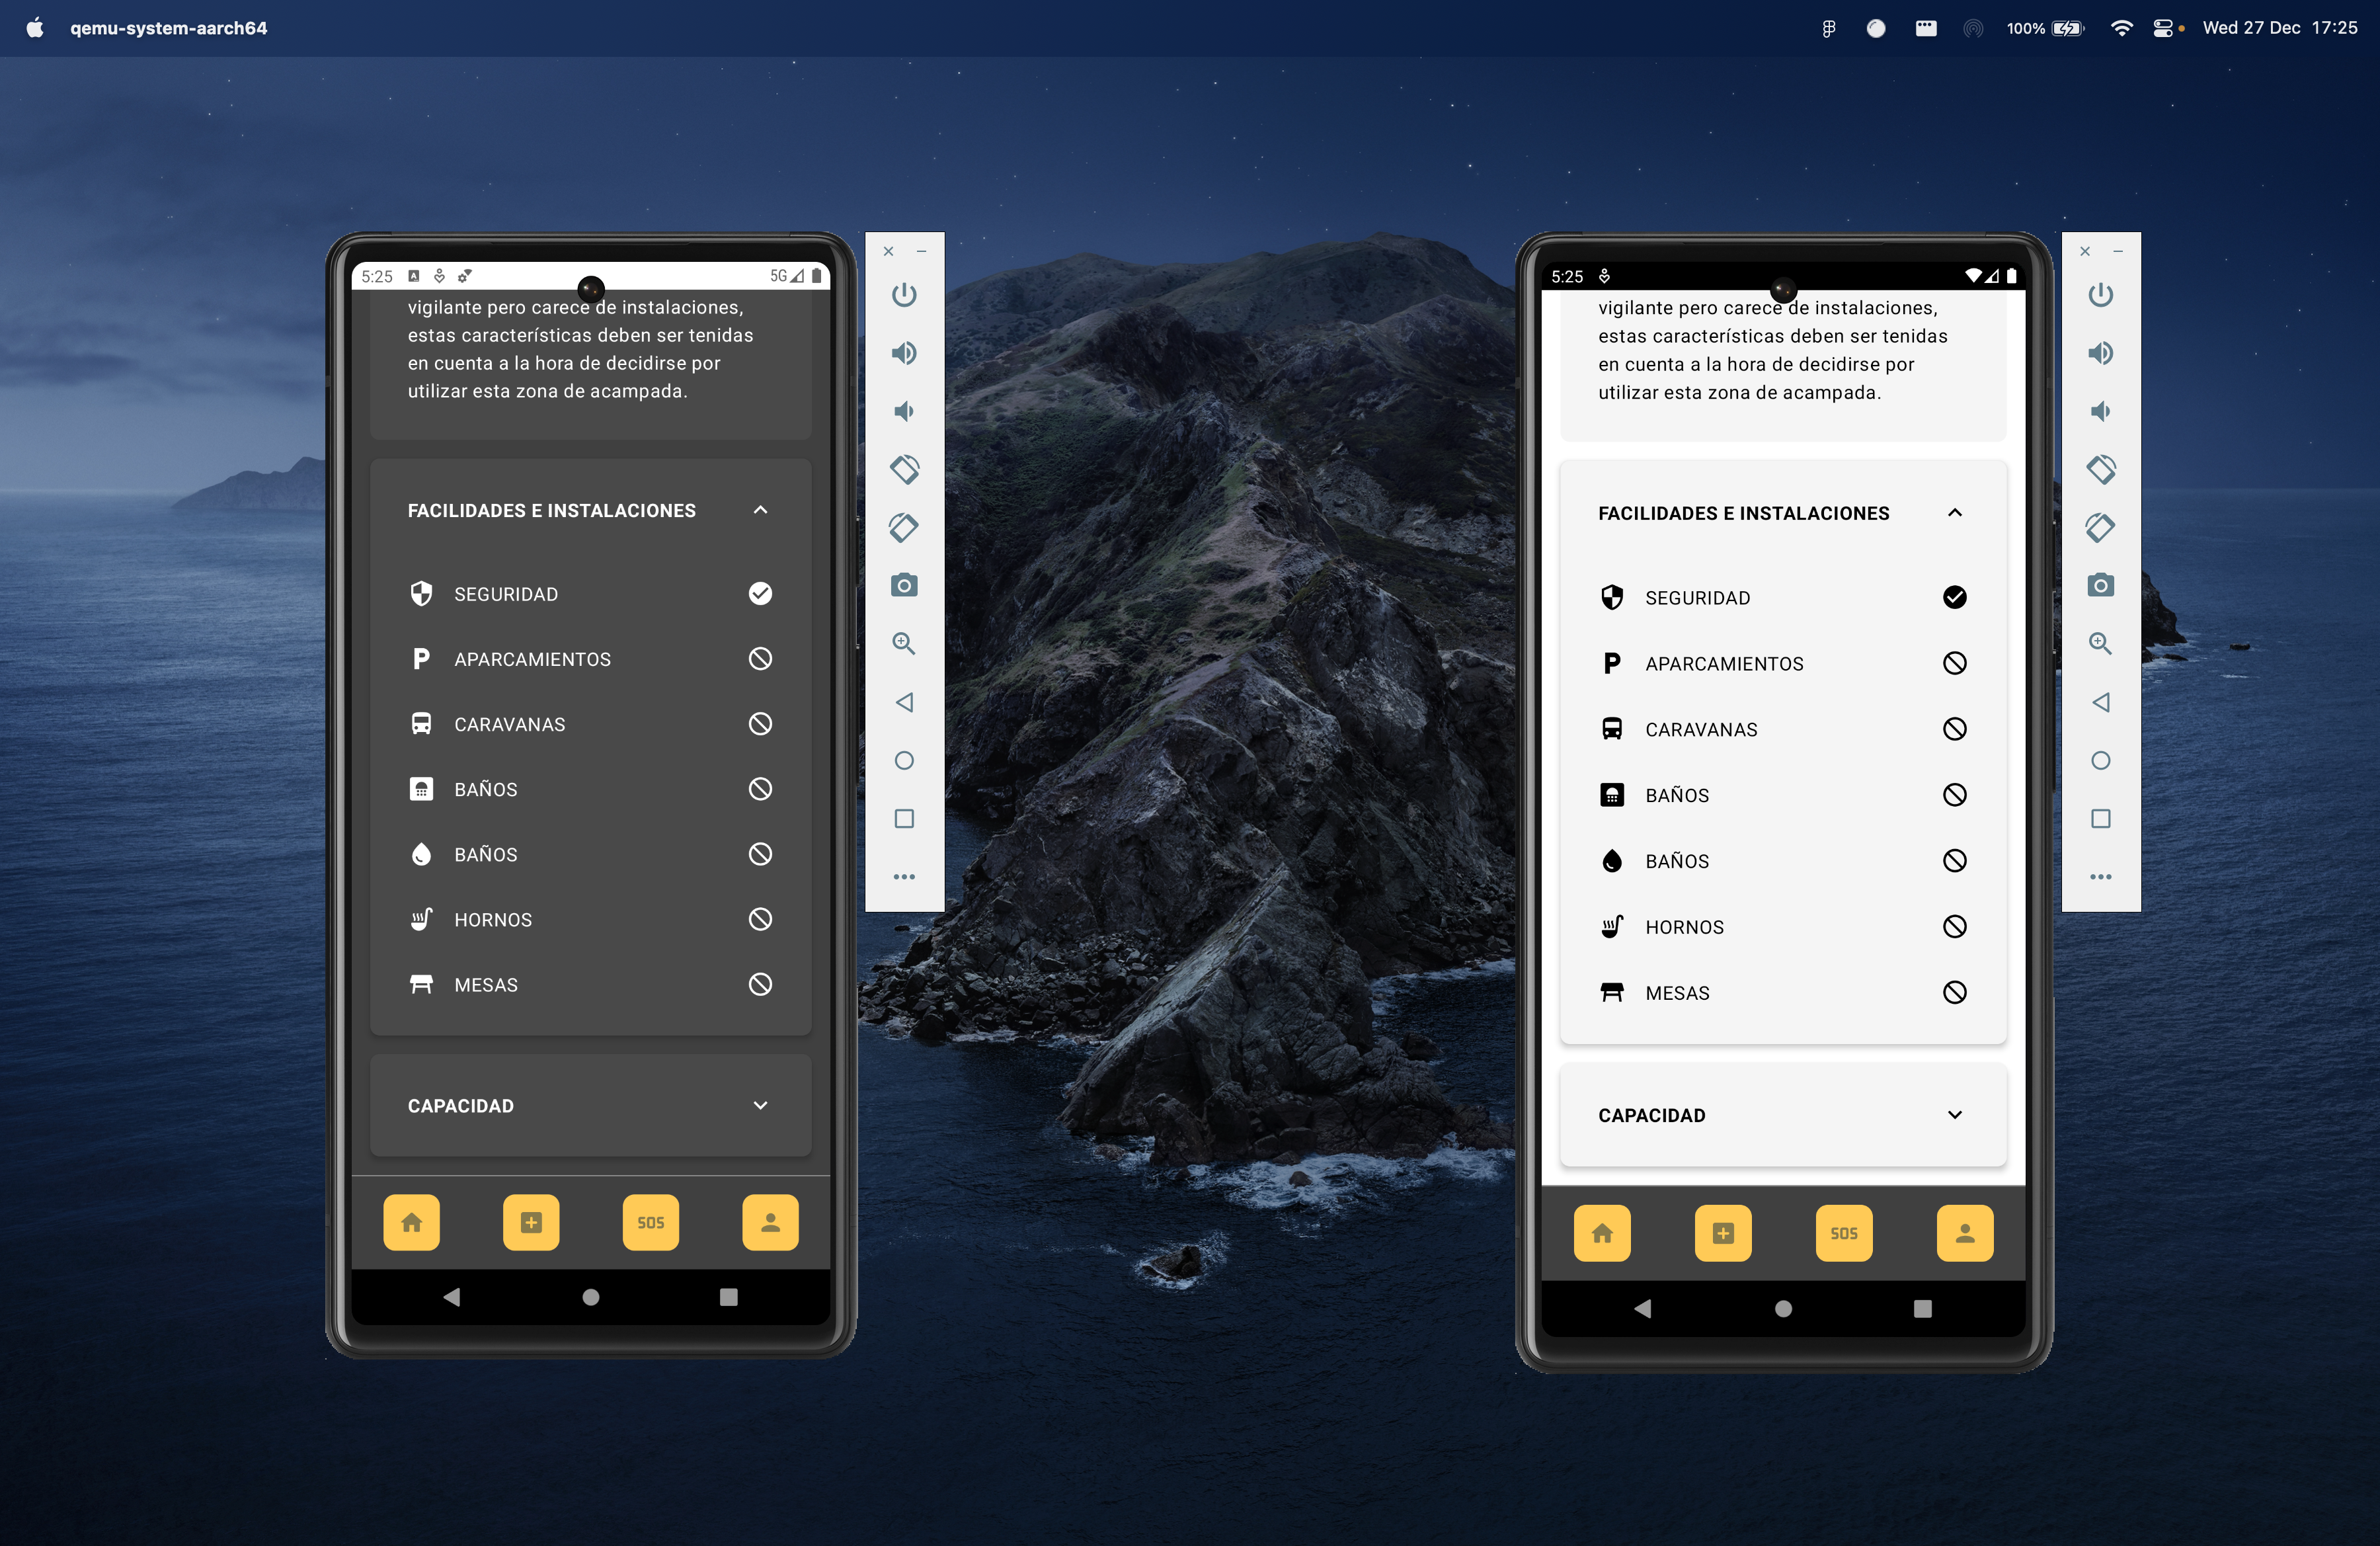
\includegraphics[scale=0.2]{area2.png}}
        \caption{Pantalla de area seleccionada con desplegable}
        \label{fig:area2}
    \end{figure}

    \begin{figure}[H]
        \centerline{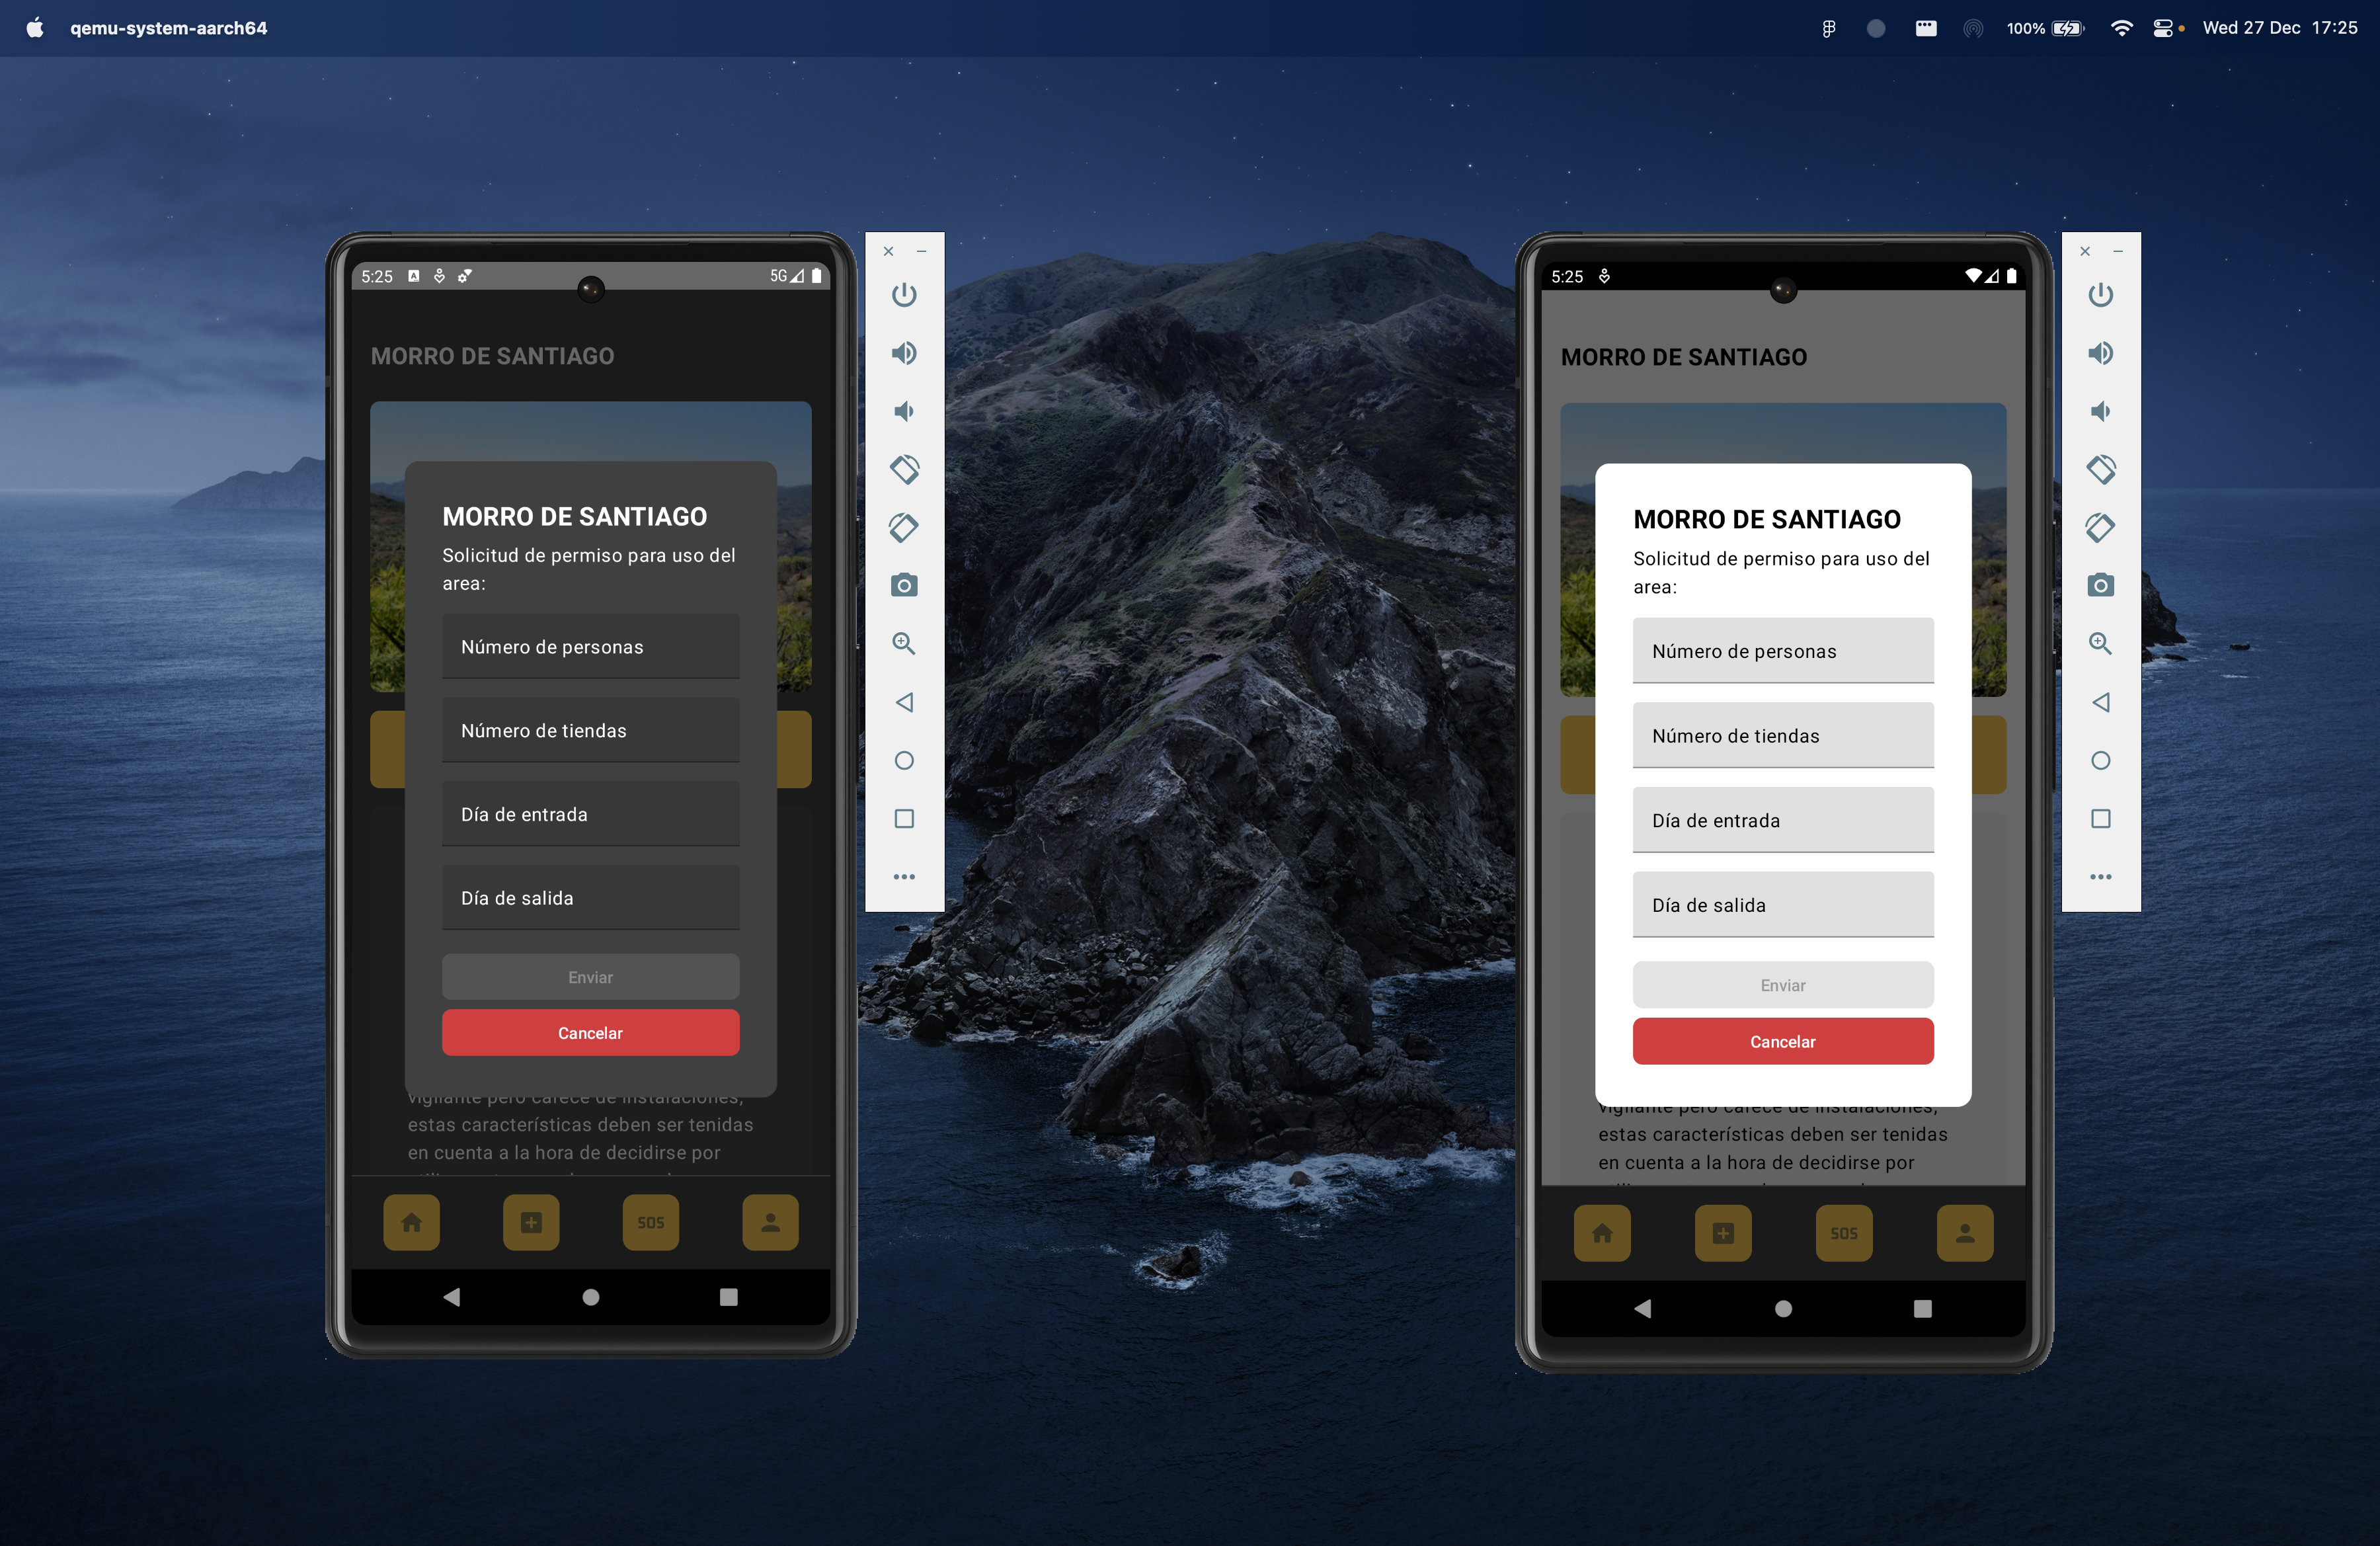
\includegraphics[scale=0.2]{area3.png}}
        \caption{Pantalla de area seleccionada, formulario de solicitud}
        \label{fig:area3}
    \end{figure}

    \begin{figure}[H]
        \centerline{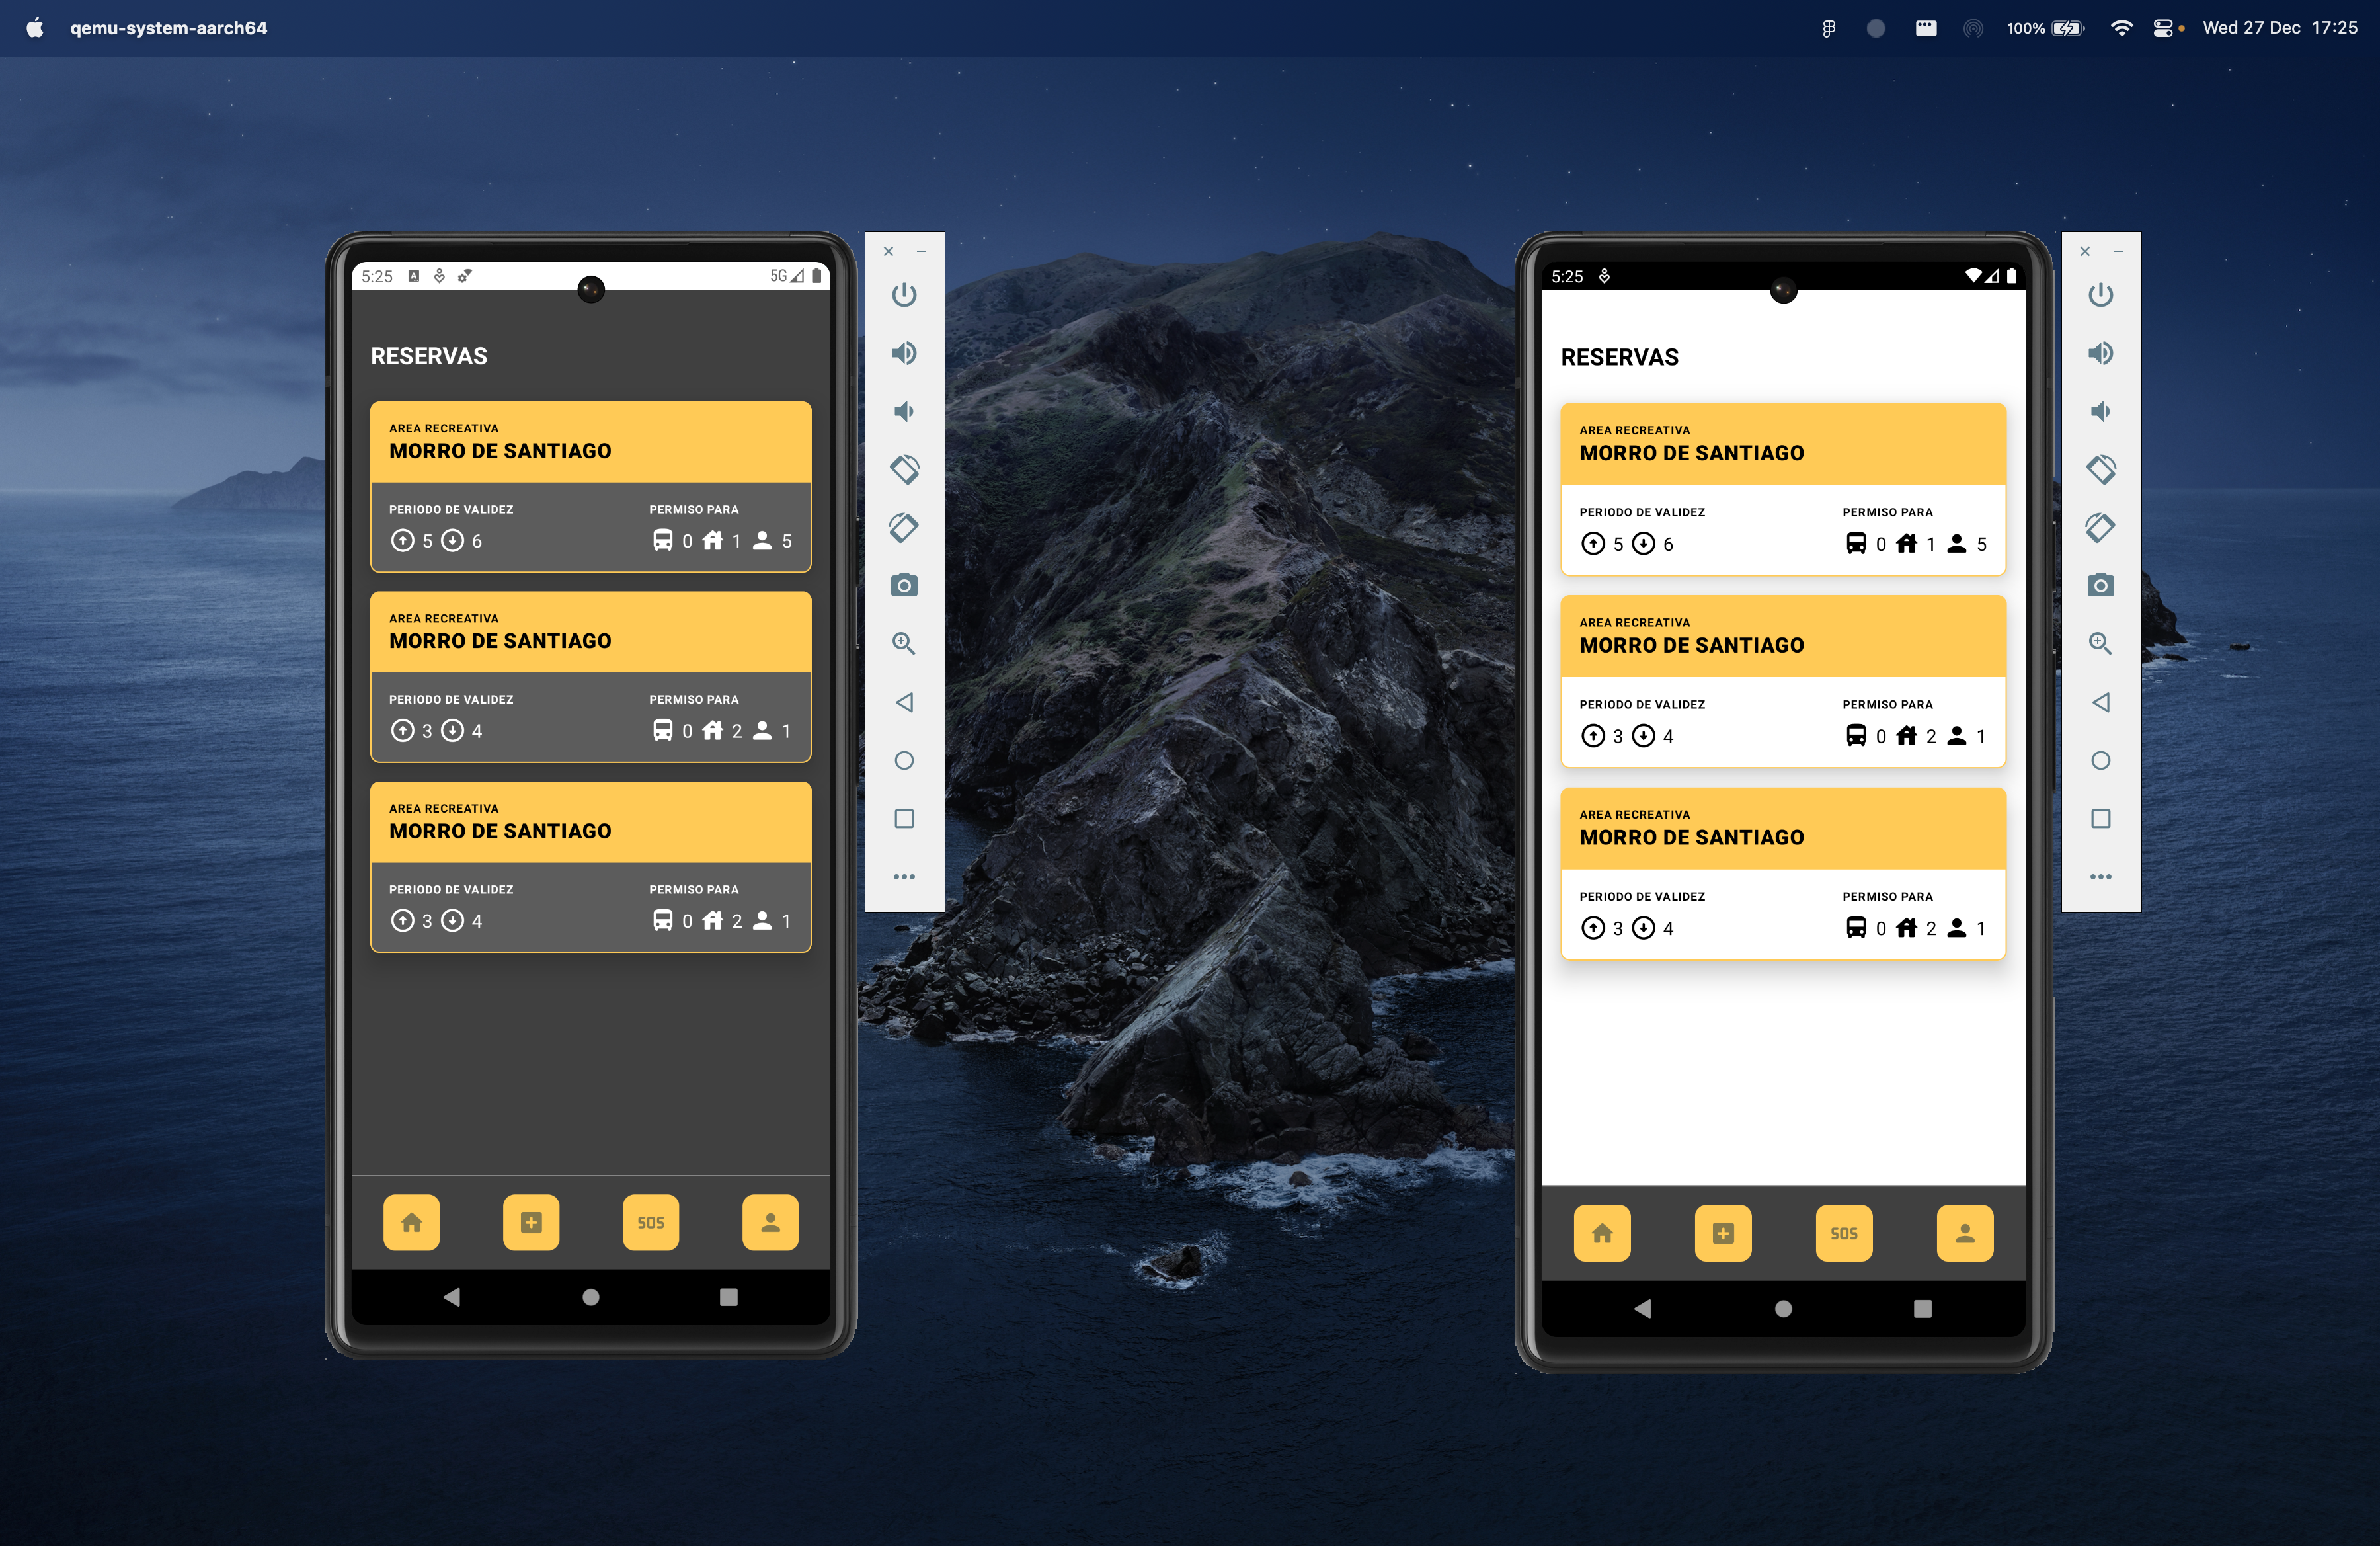
\includegraphics[scale=0.2]{book1.png}}
        \caption{Pantalla de solicitudes}
        \label{fig:book1}
    \end{figure}

    \begin{figure}[H]
        \centerline{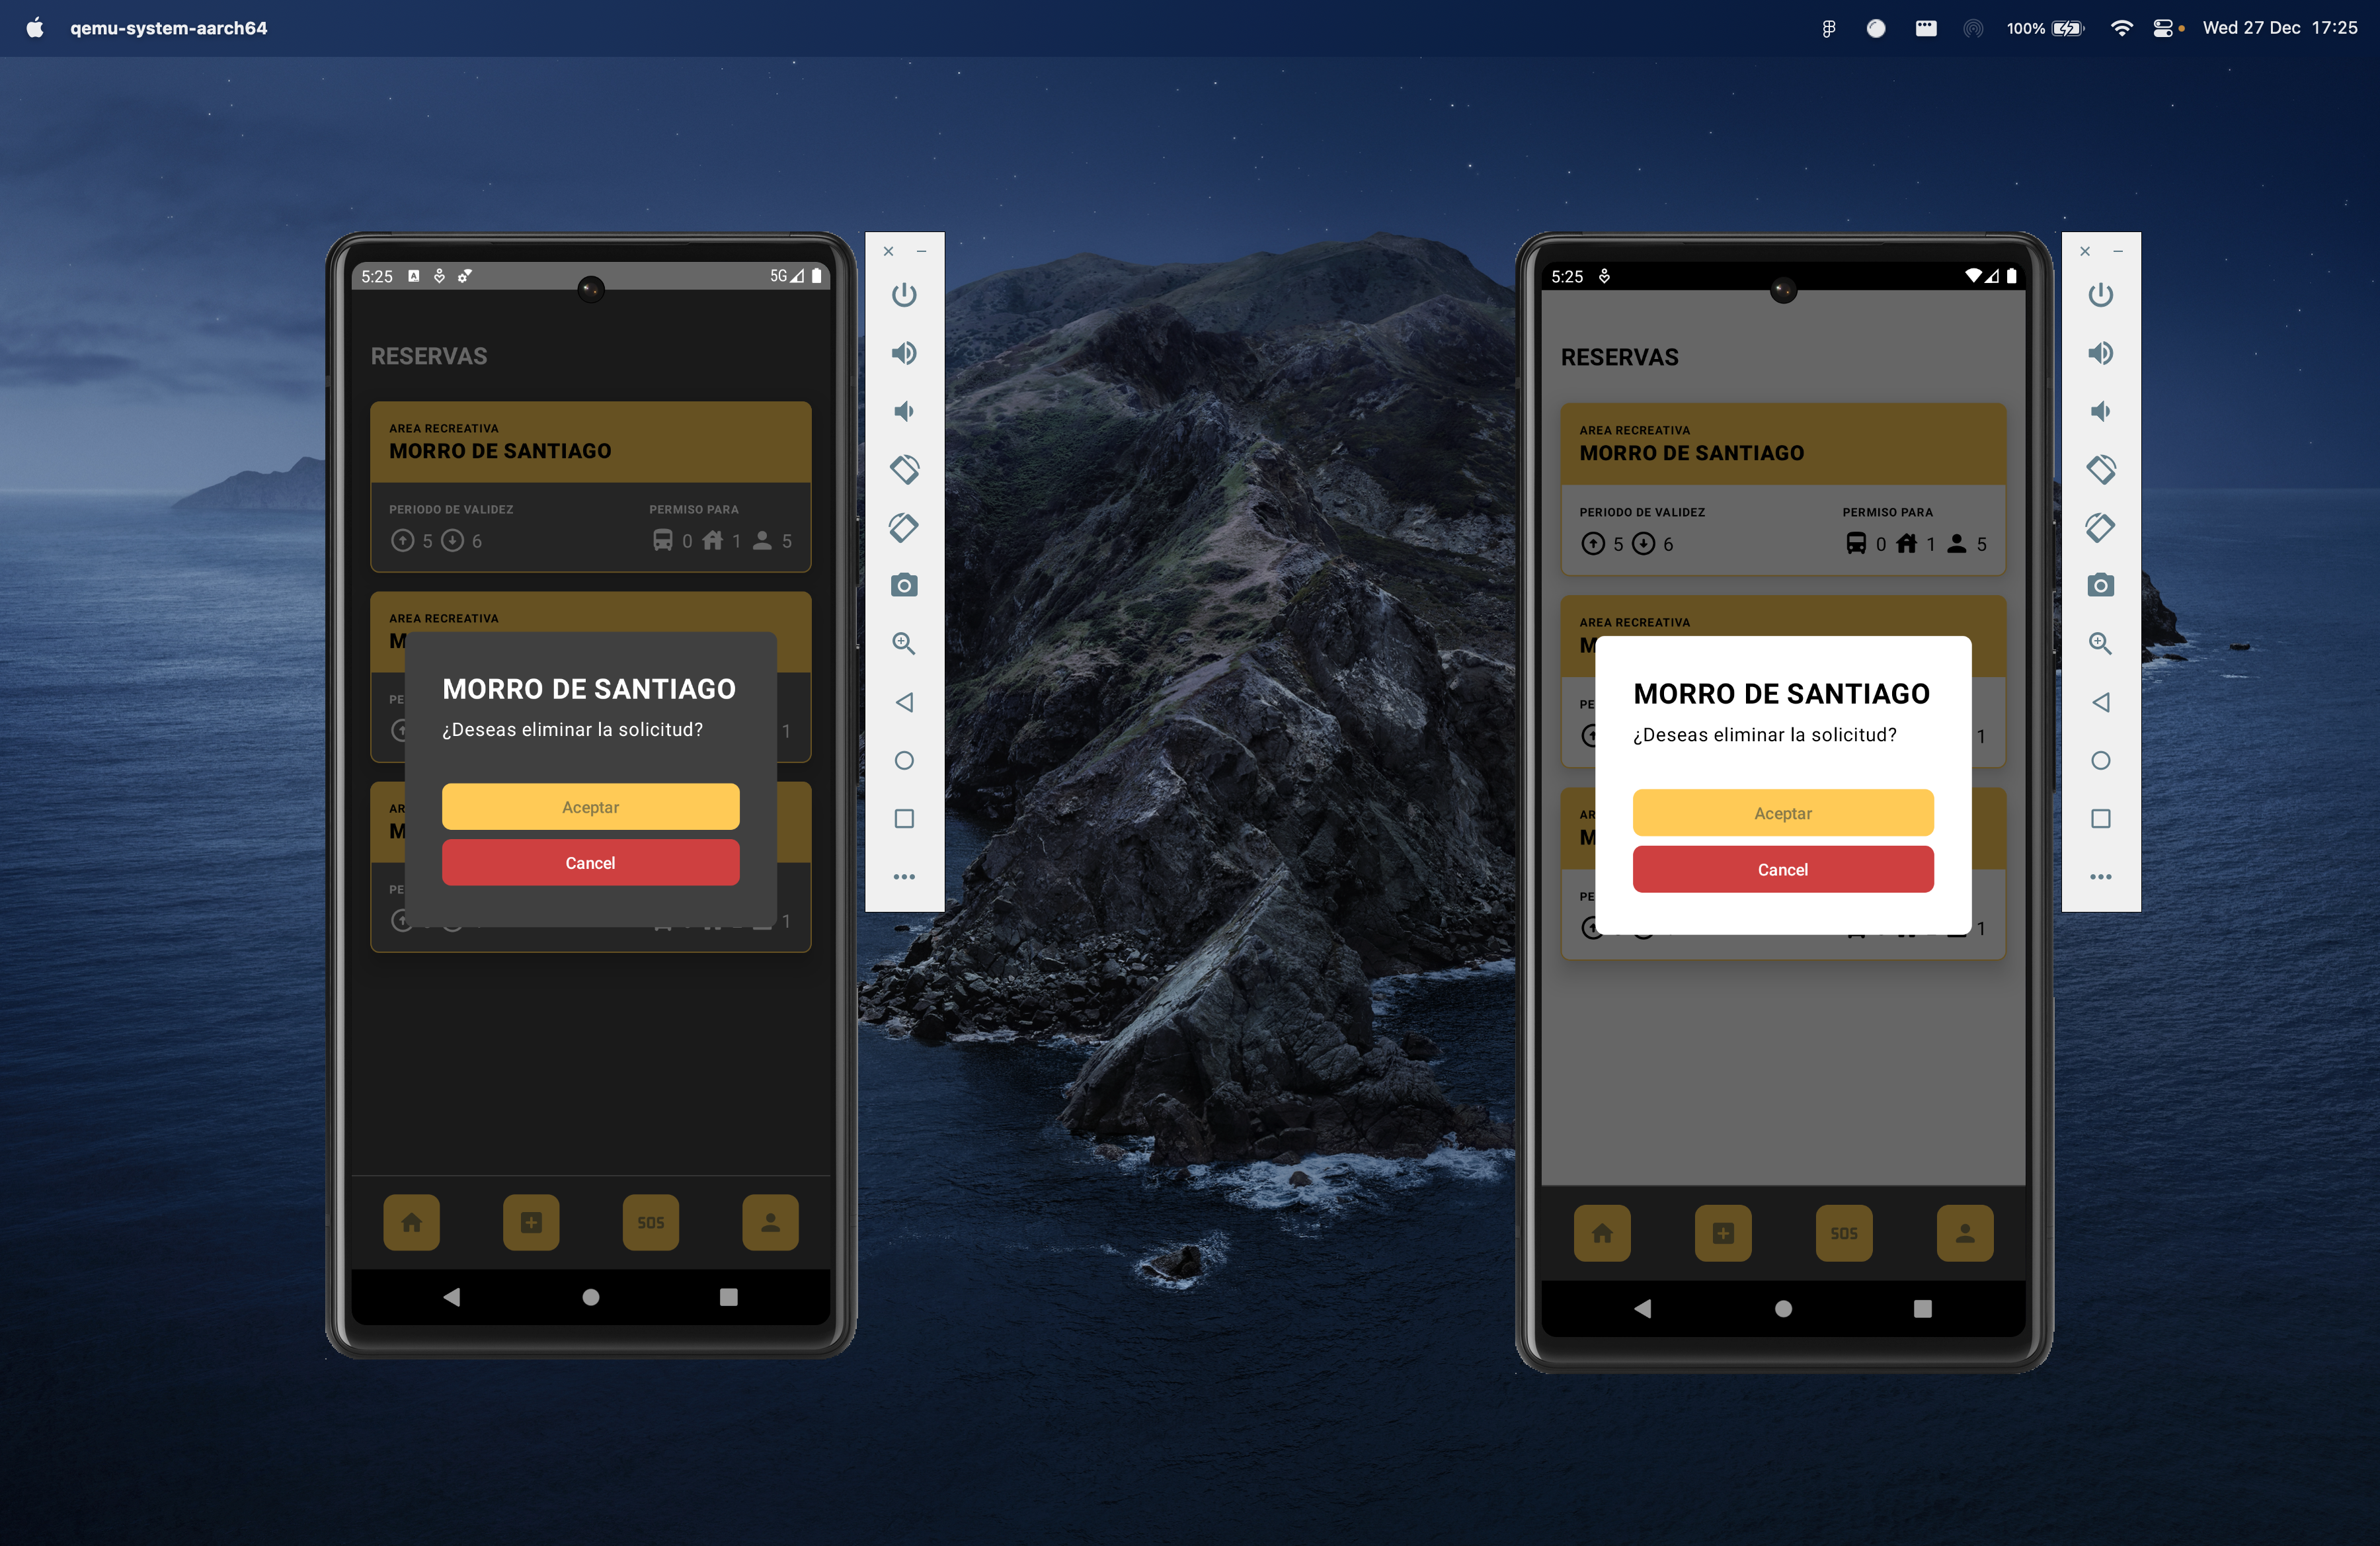
\includegraphics[scale=0.2]{book2.png}}
        \caption{Pantalla de solicitudes, formulario de eliminación}
        \label{fig:book2}
    \end{figure}

    \begin{figure}[H]
        \centerline{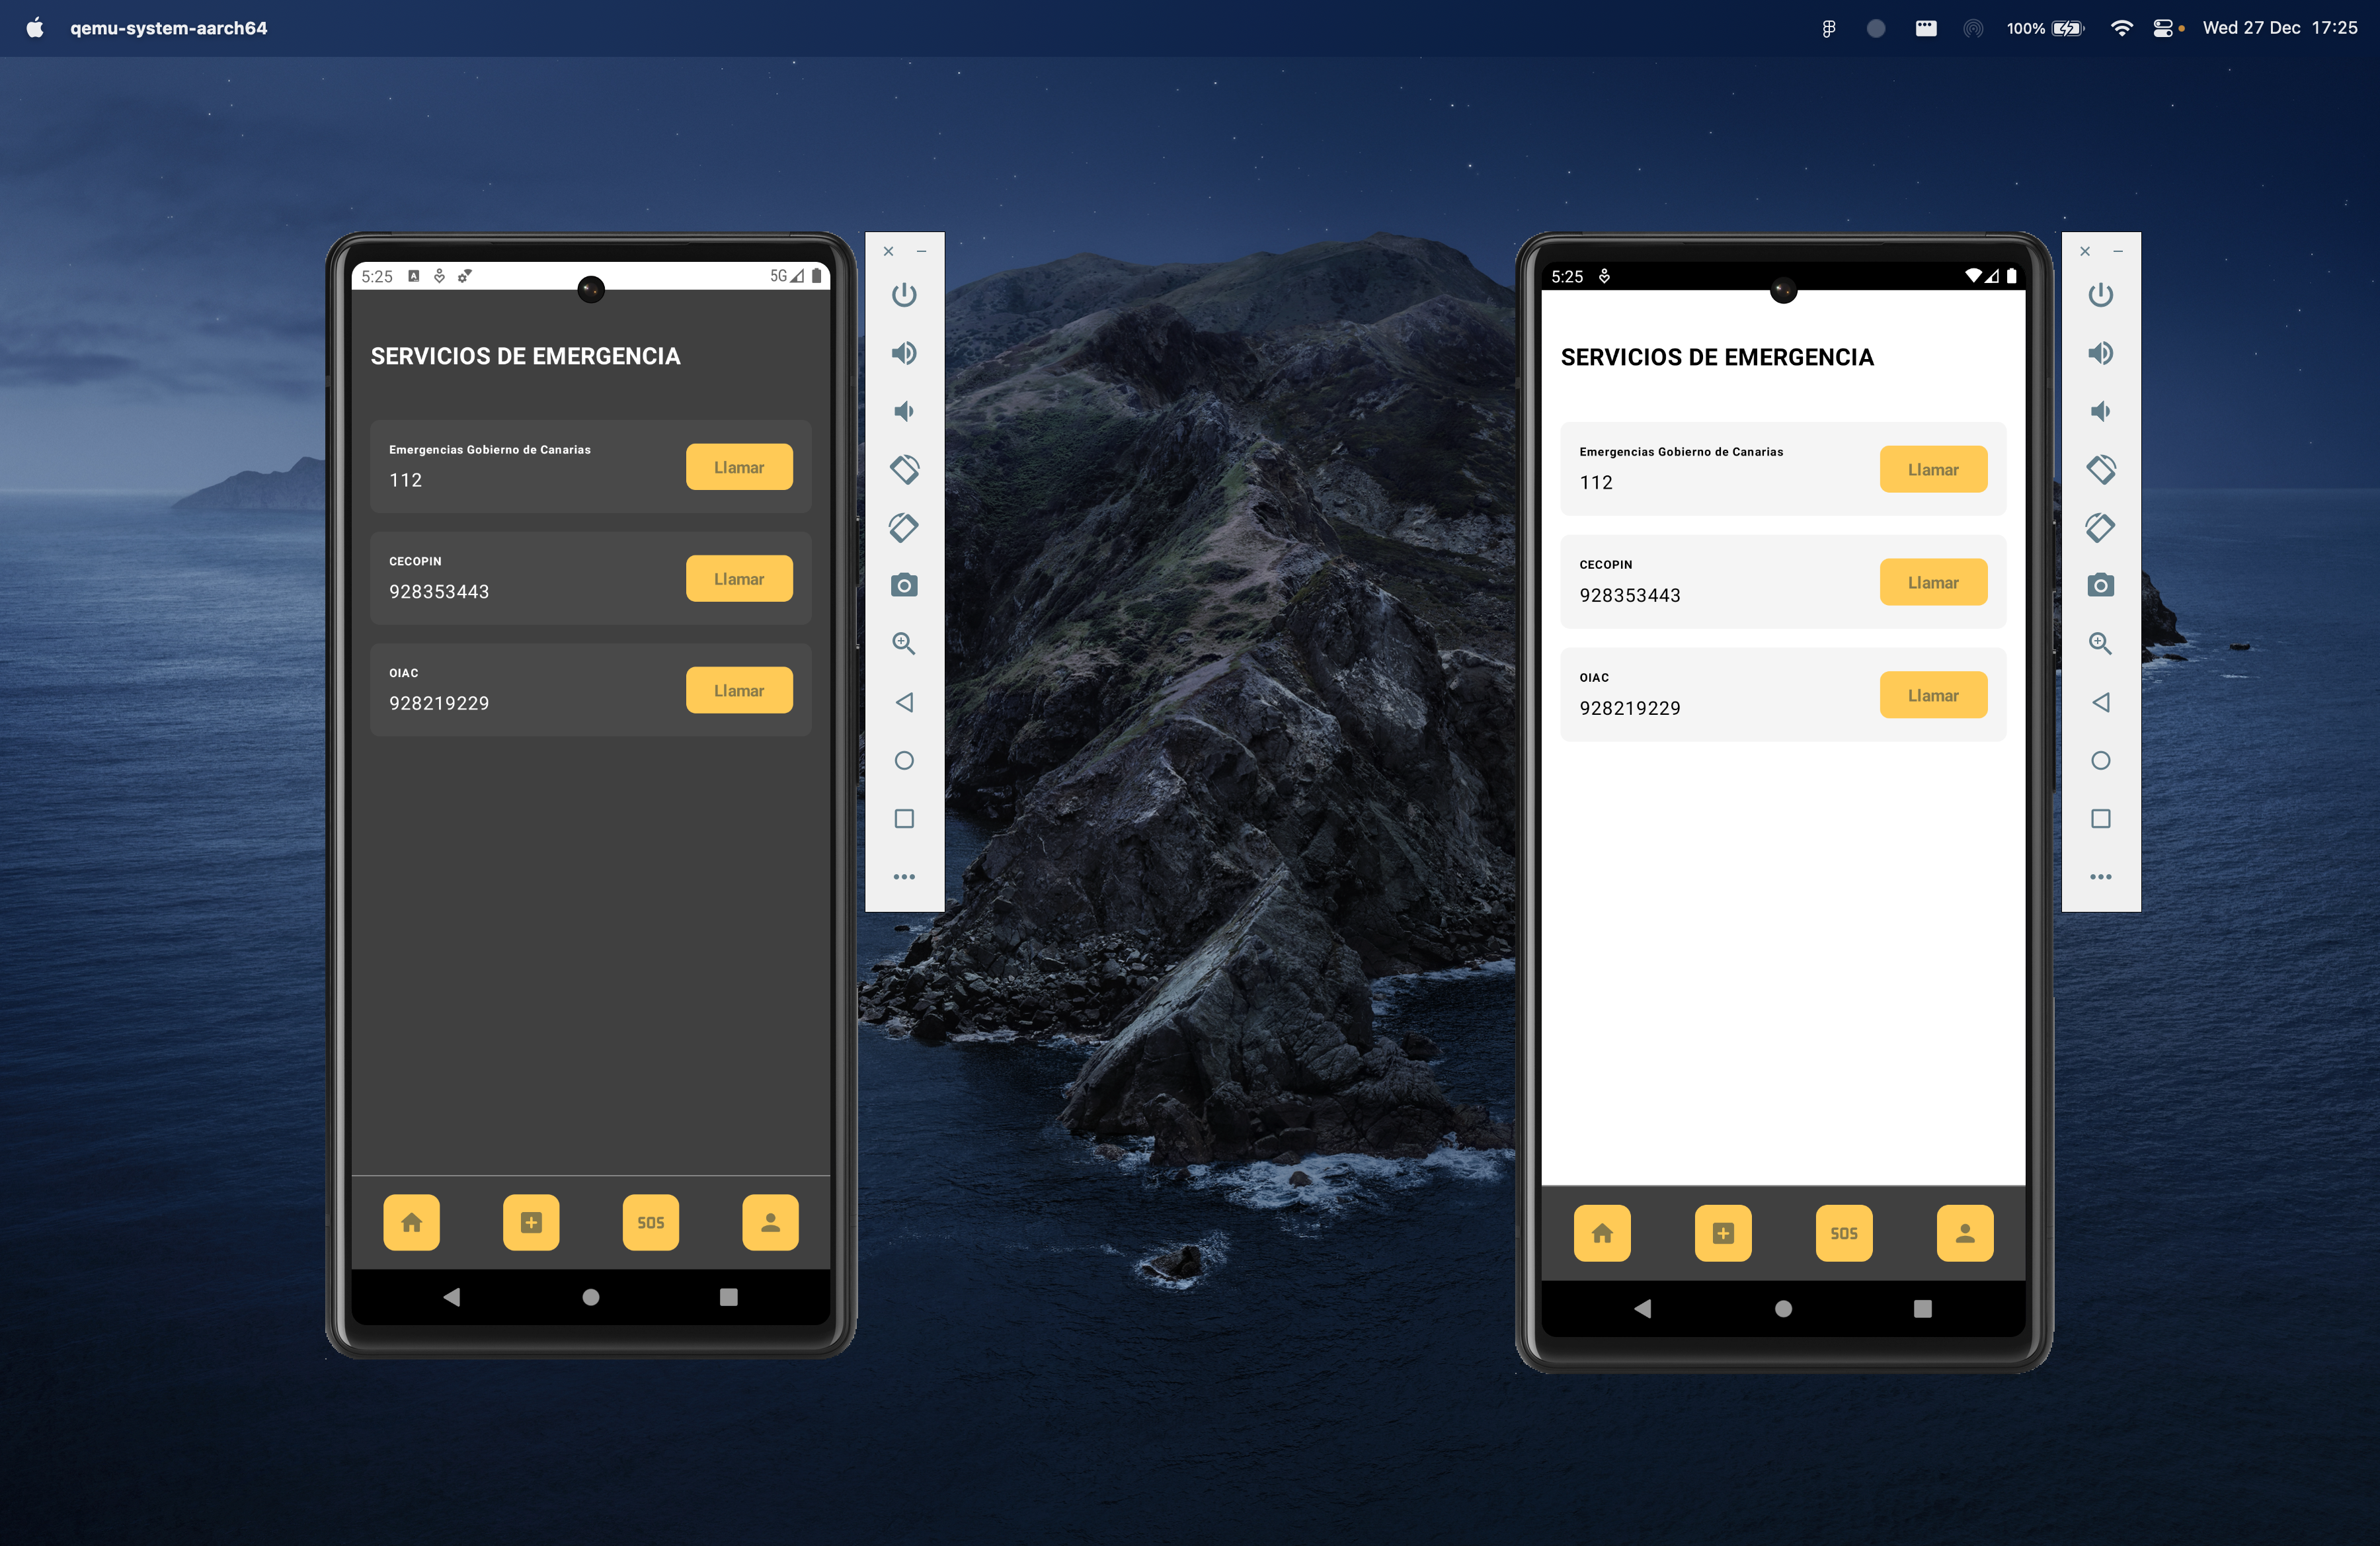
\includegraphics[scale=0.2]{emergencies.png}}
        \caption{Pantalla de emergencia}
        \label{fig:emergencies}
    \end{figure}

    \begin{figure}[H]
        \centerline{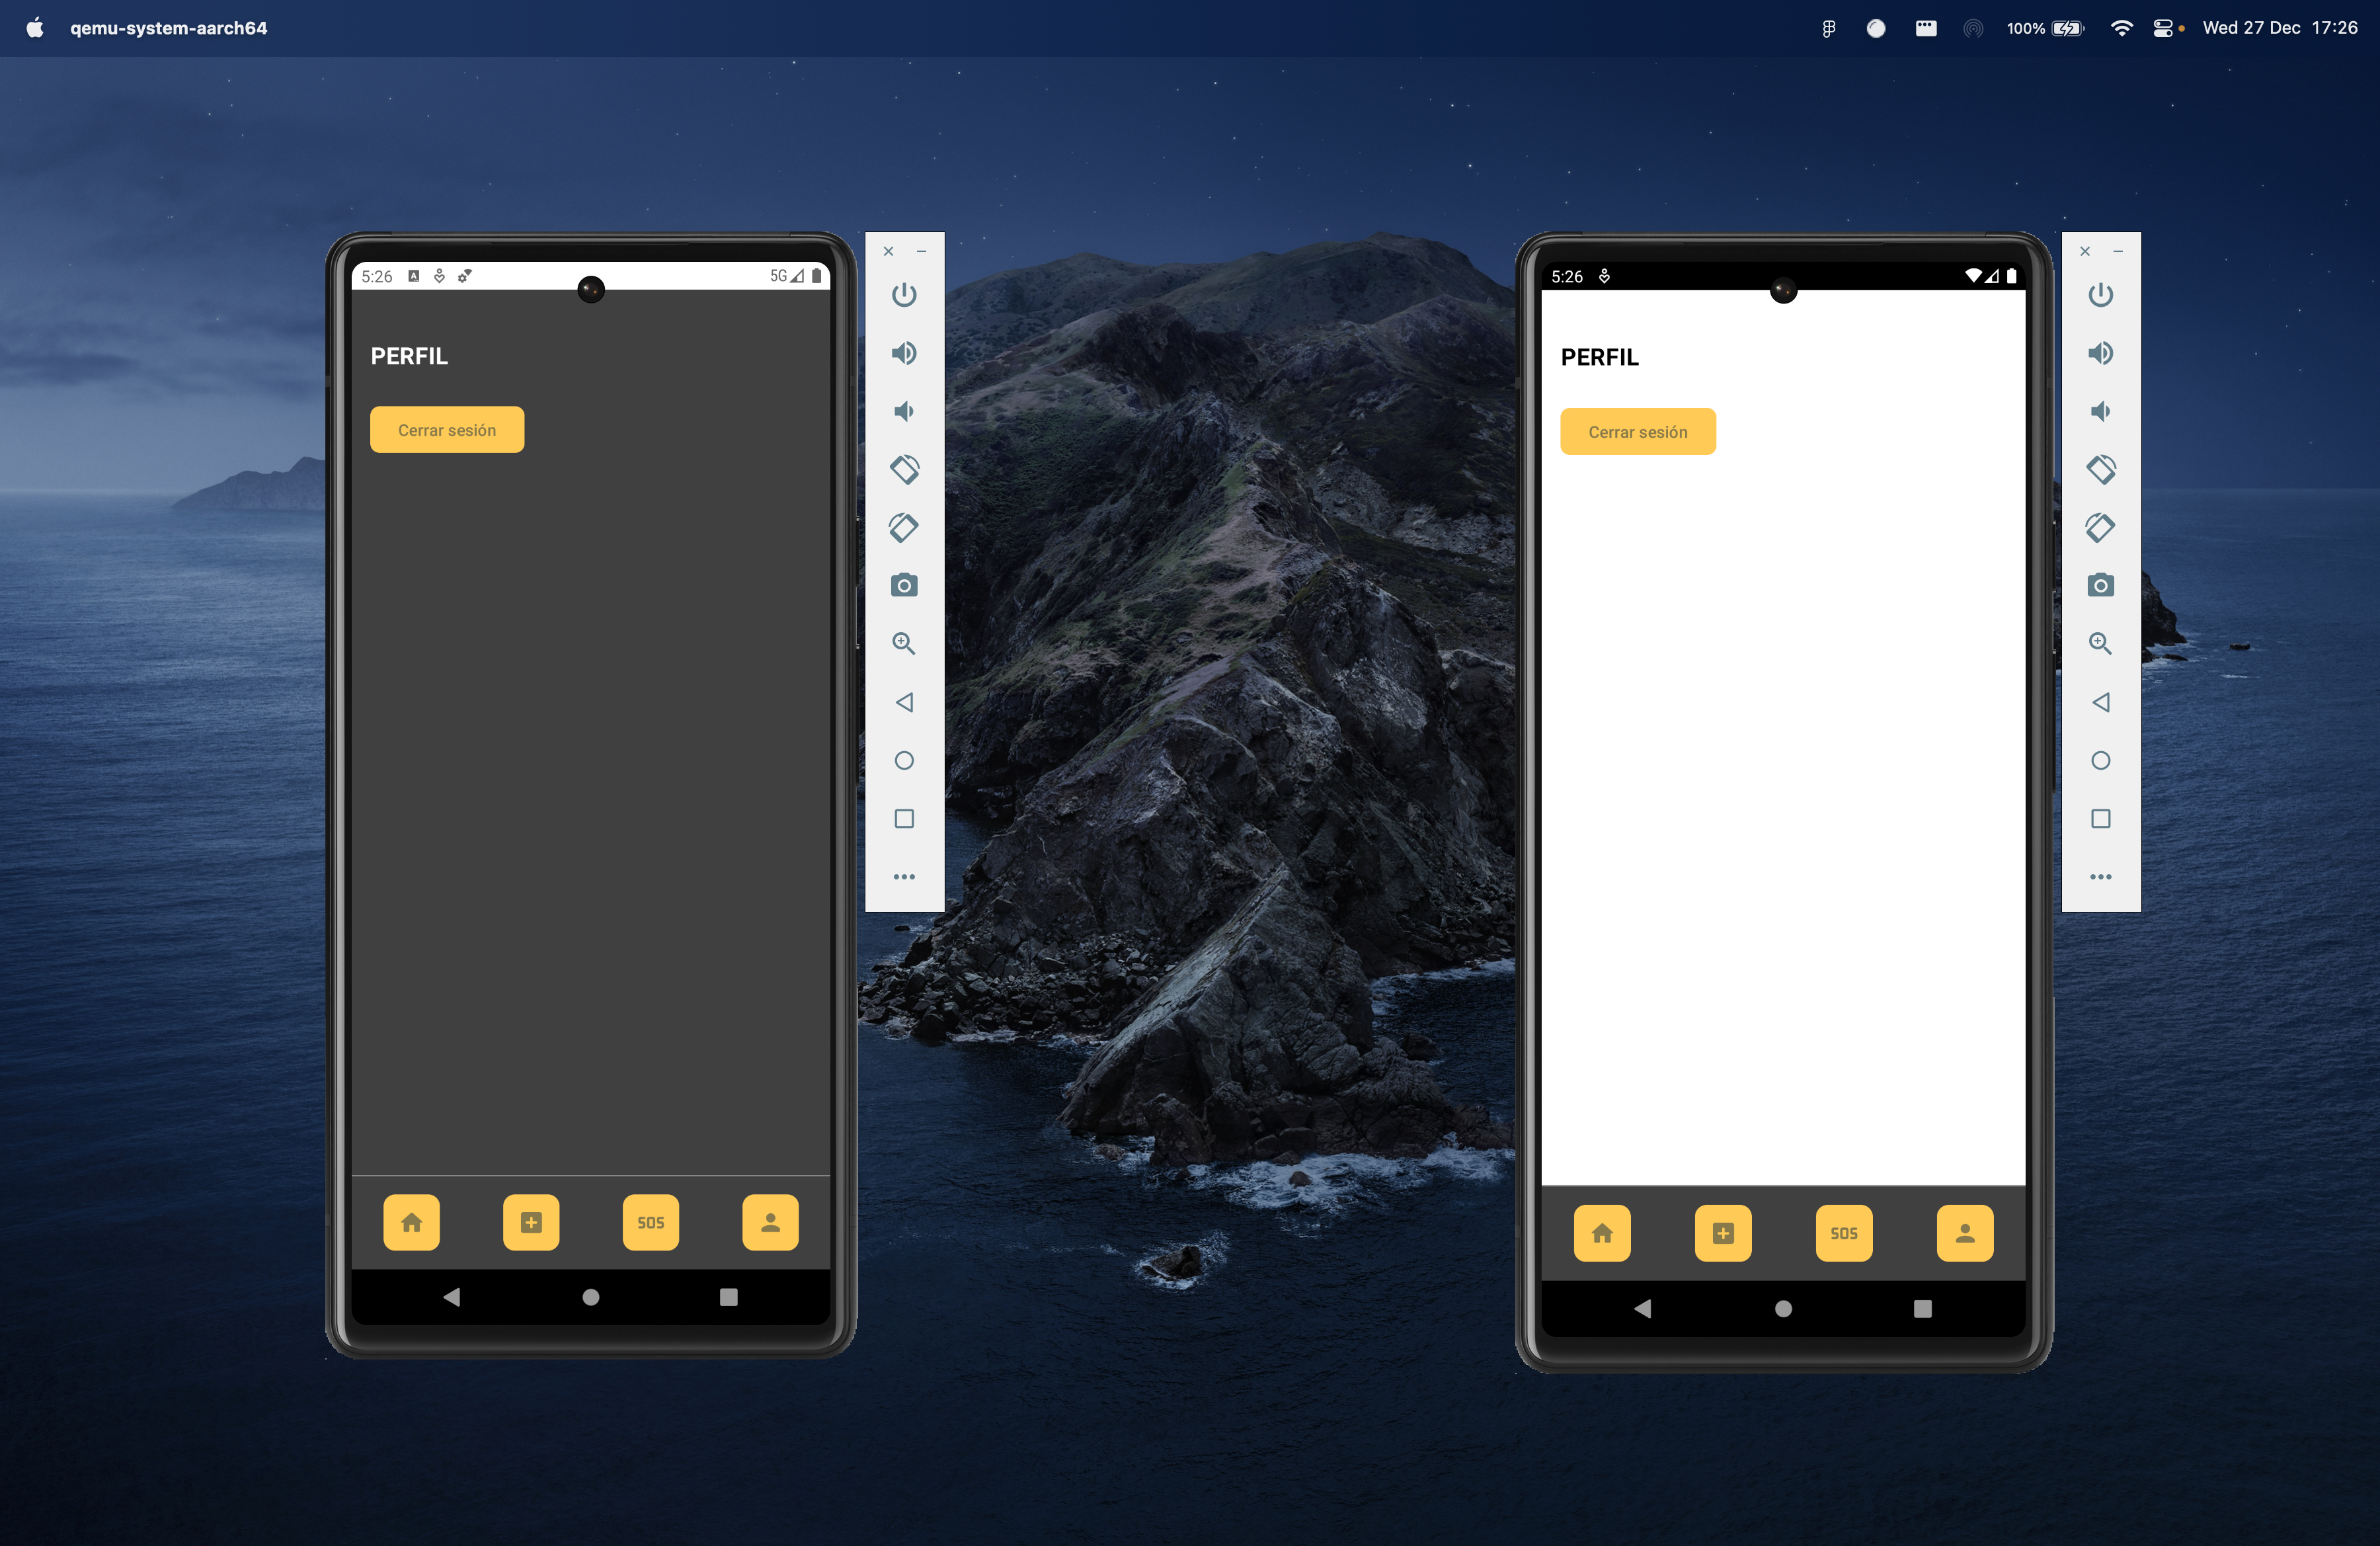
\includegraphics[scale=0.2]{profile.png}}
        \caption{Pantalla de perfil}
        \label{fig:profile}
    \end{figure}
\end{document}